\documentclass[10pt,a4paper]{article}

% ─── Packages ─────────────────────────────────────────

\usepackage{fontspec}
\setmainfont{Times New Roman}

\usepackage[top=1.0cm,bottom=0.9cm,left=1.45cm,right=1.45cm]{geometry}

\usepackage{titlesec}
\usepackage{enumitem}
\usepackage{hyperref}
\usepackage{xcolor}
\usepackage{tabularx}
\usepackage{graphicx}
\usepackage{parskip}

% ─── Colors ───────────────────────────────────────────

\definecolor{primary}{RGB}{30,40,90}
\definecolor{namecolor}{RGB}{0,120,180}
\definecolor{accent}{RGB}{50,90,150}
\definecolor{rulecol}{RGB}{200,205,220}
\definecolor{gray}{RGB}{90,90,90}

\hypersetup{
    colorlinks=true,
    urlcolor=accent
}

\pagestyle{empty}
\setlength{\parskip}{0pt}

% ─── Section ──────────────────────────────────────────

\titleformat{\section}
    {\normalsize\bfseries\color{primary}}
    {}
    {0em}
    {}
    [\vspace{1pt}\textcolor{rulecol}{\titlerule[0.6pt]}\vspace{1pt}]

\titlespacing{\section}{0pt}{4pt}{2pt}

% ─── Entry ────────────────────────────────────────────

\newcommand{\entry}[3]{%
    \noindent
    \begin{tabularx}{\linewidth}{X r}
        \textbf{\color{primary}#1} &
        {\scriptsize\color{gray}#2}
    \end{tabularx}\\[-2pt]
    {\scriptsize\textit{\color{gray}#3}}
    \vspace{0.5pt}
}

% ─── Compact list ─────────────────────────────────────

\newenvironment{cvitems}{
    \begin{itemize}[
        leftmargin=1.1em,
        topsep=0pt,
        itemsep=0.3pt,
        parsep=0pt,
        partopsep=0pt
    ]
}{
    \end{itemize}
}

% ═════════════════════════════════════════════════════

\begin{document}

% ─── HEADER ───────────────────────────────────────────

\noindent

\begin{tabularx}{\linewidth}{@{}X r@{}}

\begin{minipage}[c]{\linewidth}

    {\LARGE\bfseries\color{namecolor} Ho Huynh Nhu}\\[1pt]

    {\large\bfseries\color{primary}
    Data Analyst}\\[2pt]

    {\scriptsize\color{gray}
    20/10/2003
    \enspace\textcolor{rulecol}{|}
    \enspace (+84) 367 503 477
    \enspace\textcolor{rulecol}{|}
    \enspace
    \href{mailto:hhnhu2003@gmail.com}{hhnhu2003@gmail.com}
    \enspace\textcolor{rulecol}{|}
    \enspace Ho Chi Minh City}\\[1pt]

    {\scriptsize
    \href{https://github.com/hohuynhnhu}
    {github.com/hohuynhnhu}
    \enspace\textcolor{rulecol}{|}
    \enspace
    \href{https://www.facebook.com/huynhnhu.ho.961}
    {facebook.com/huynhnhu.ho.961}
    }

\end{minipage}

&

\begin{minipage}[c]{2.1cm}
    \raggedleft
    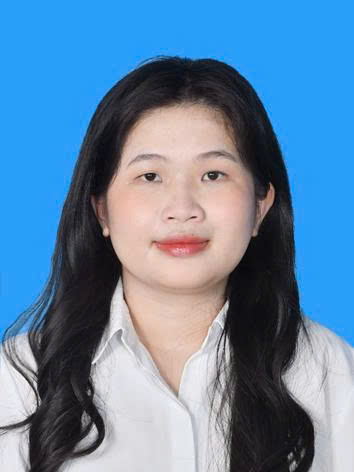
\includegraphics[
        width=2.1cm,
        height=2.5cm,
        keepaspectratio
    ]{assets/avt.jpg}
\end{minipage}

\end{tabularx}

\vspace{2pt}

\textcolor{rulecol}{\rule{\linewidth}{0.6pt}}

% ─── CAREER OBJECTIVE ─────────────────────────────────

\section*{Career Objective}

{\small
Final-year Information Technology student pursuing a career in Data
Analysis, with hands-on experience in SQL, Python, data processing,
ETL, and Power BI. Experienced in cleaning and transforming
operational data, building analytical datasets, developing dashboards,
and analyzing data to identify trends and operational insights.
Seeking a Data Analyst position to apply analytical skills to
real-world business problems and support data-driven decision-making.
}

% ─── EDUCATION ────────────────────────────────────────

\section*{Education}

\entry
{University of Transport Ho Chi Minh City (UTH)}
{10/2022 -- 10/2026}
{Bachelor of Information Technology -- Completed coursework}

{\small
\begin{cvitems}

    \item GPA: \textbf{3.4 / 4.0}

    \item \textbf{Excellent Scholarship} -- Semester 1, 2025

    \item \textbf{Second Prize -- AI Track},
    UTH Student Scientific Research Conference 2025

\end{cvitems}
}

% ─── TECHNICAL SKILLS ─────────────────────────────────

\section*{Technical Skills}

{\small

\begin{tabularx}{\linewidth}{@{}lX@{}}

\textbf{Data Analysis}
&
Data Cleaning, Data Transformation, Data Validation,
Exploratory Data Analysis, KPI Analysis, Trend Analysis
\\[1pt]

\textbf{SQL}
&
SQL, PostgreSQL, SQL Server, MySQL, Joins, CTEs,
Aggregations, Subqueries, Window Functions
\\[1pt]

\textbf{BI / Visualization}
&
Power BI, DAX, Dashboard Development, Data Visualization,
Operational Reporting
\\[1pt]

\textbf{Excel}
&
Excel, Data Cleaning, Data Filtering, Pivot Tables,
Lookup Functions, Reporting
\\[1pt]

\textbf{Python}
&
Python, Pandas, NumPy, Matplotlib, Data Processing,
Data Analysis Automation
\\[1pt]

\textbf{ETL / Data}
&
ETL/ELT, dbt, Apache Airflow, Data Pipeline,
Data Modeling, Data Warehouse
\\[1pt]

\textbf{Databases}
&
PostgreSQL, SQL Server, MySQL, MongoDB,
Firebase, Supabase, Neon PostgreSQL
\\[1pt]

\textbf{Tools}
&
Git, Docker, Postman, VS Code, Jira, Confluence

\end{tabularx}

}

% ─── WORK EXPERIENCE ──────────────────────────────────

\section*{Work Experience}

\entry
{Gotik Consulting -- Data Engineer}
{Python \textbar{} dbt \textbar{} PostgreSQL \textbar{} Airflow \textbar{} Power BI}
{03/2026 -- 05/2026}

{\small
\begin{cvitems}
    \item Processed and transformed Odoo business data using Python and SQL to prepare clean and structured datasets for analytics and reporting.
    
    \item Built Python-based ETL pipelines to extract data from source systems, perform data cleaning and transformation, and load processed data into Neon PostgreSQL.
    
    \item Developed dbt models to transform raw data into structured analytical datasets, improving data consistency and making datasets easier to maintain and reuse.
    
    \item Designed and automated hourly data workflows with Apache Airflow, including task scheduling, dependency management, and monitoring of ETL processes.
    
    \item Built Power BI dashboards to visualize operational and business metrics, providing interactive reports for monitoring performance and supporting data-driven analysis.
    
    \item Wrote SQL queries for data aggregation, filtering, joins, and analytical reporting, ensuring reliable data sources for downstream dashboards and business analysis.
\end{cvitems}
}

% ─── PROJECTS ─────────────────────────────────────────

\section*{Featured Data Projects}

\entry
{Delivery Driver -- Order Analytics System}
{Python \textbar{} SQL \textbar{} Kafka \textbar{} PostgreSQL \textbar{} Power BI}
{12/2025 -- 02/2026}

{\small
\begin{cvitems}
    \item Built an automated data pipeline with Data Lake and Data Warehouse to collect, process, and prepare order data for analysis.
    \item Applied RFM and Association Rule Mining to analyze customer behavior and identify frequent pickup--delivery location patterns.
    \item GitHub: \href{https://github.com/LeKhang-cn22h/BE-delivery-driver}{BE-delivery-driver}
\end{cvitems}
}

\vspace{2pt}

\entry
{VehicleScan -- Smart Parking Data System}
{Python \textbar{} SQL \textbar{} PostgreSQL \textbar{} Firebase \textbar{} ESP32}
{03/2025 -- 03/2026}

{\small
\begin{cvitems}
    \item Collected and processed vehicle and IoT sensor data using Python and SQL for real-time parking management.
    \item Integrated AI, sensor, and application data into a centralized system to support monitoring and data analysis.
    \item GitHub: \href{https://github.com/LeKhang-cn22h/VehicleScanner}{VehicleScanner}
\end{cvitems}   
}

% ─── ADDITIONAL INFORMATION ───────────────────────────

\section*{Additional Information}

{\small

\begin{tabularx}{\linewidth}{@{}lX@{}}

\textbf{English}
&
Technical document reading and basic professional communication

\\[1pt]

\textbf{Availability}
&
Available for full-time Data Engineer opportunities.

\end{tabularx}

}
\end{document}